\documentclass[12pt, a4paper]{article}
% \usepackage{mathtools}
\usepackage{graphicx}
\usepackage{amsthm}
\usepackage{hyperref}
\usepackage{amssymb}
\graphicspath{{images/}}

\hypersetup{
    colorlinks=true,
    linkcolor=blue,
    urlcolor=cyan
}

\title{AP Stats Notes}
\author{Franklin Chen}
\date{11 November 2024 - idk some time in may}

\theoremstyle{definition}
\newtheorem{definition}{Definition}

\begin{document}
\maketitle
\newpage
% comment

\tableofcontents
\newpage

using \textit{The Practice of Statistics for the AP Exam: 6th Edition} by Starnes and Tabor

\section{Data Analysis}
\subsection{What is Statistics?}

\begin{definition}[Statistics]
    The science of collecting, analyzing, and drawing conclusions from data.
\end{definition}

Data is collected from \emph{individuals} about certain \emph{variables}.

\begin{definition}[Individual, Variable]
    
    \textbf{Individuals} are objects described in a dataset. Typically people, but not always.
    
    \textbf{Variables} are attributes that can take different values for different individuals.
\end{definition}

For example, \emph{individuals} may be households, and \emph{variables} may be region, nnumber of people, household income, etc. It's important to distinguish between \emph{categorial} and \emph{quantative} variables:

\begin{definition}[Categorical and Quantative Variables]
    \textbf{Categorical Variables} are variables whose values can be placed into distinct categories.

    \textbf{Quantative Variables} are variables whose values are quantities, typically counts or measurements.
\end{definition}

For example, region would be categorical, while household income would be quantative. \emph{Not all numbers are quantative}; eg. zip code.

\subsection{Analyzing Categorical Data}
\subsubsection{One-Variable Categorical Data}
\begin{definition}[Frequency and Relative Frequency Tables]
    \textbf{Frequency Tables}shows the number of individuals that have values of a certain category. \textbf{Relative Frequency Tables} shows the proportion or percent of individuals in each category.
\end{definition}

\emph{Note (relative) frequencies are not data; they \emph{summarize} data.} Bar graphs and Pie Graphs summarize relative frequency tables.

\emph{Beware of misleading graphs}; we mainly react to the area of each bar, not the actual height.

\subsubsection{Two-Variable Categorical Data}
Use a two-way table to summarize data about two categorical variables. These tables can be used to answer questions about \emph{marginal, joint, and conditional relative frequencies.}
\begin{figure}[t]
    \centering
    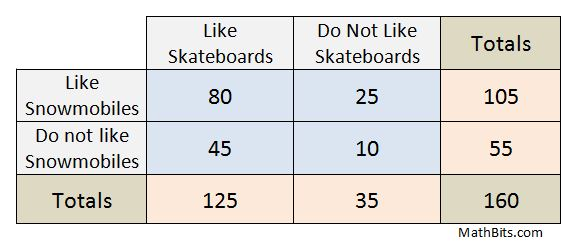
\includegraphics[width=0.75\textwidth]{two way table.png}
    \caption{An example two-way table with additional summary information.}
    \label{fig:two-way-table}
\end{figure}

\textbf{Margial relative frequencies} give the percent or proportion of individuals that have a given value for one categorical variable. For example, the marginal relative frequency of liking skateboards is $\frac{125}{160} \approx 78.125\%$.

\textbf{Joint relative frequencies} give the percent or proportion of individuals that have a specific value for both categorical variables. For example, the joint frequency of liking both skateboards and snowmobiles is $\frac{80}{160} = 50\%$.

\textbf{Conditional relative frequencies} give the percent or proportion of individuals that have a specific value for one categorical variable relative to other individuals with the same other categorical variable. For example, the conditional relative frequency of those who like snowmobiles out of all individuals that like skateboards is $\frac{80}{125} = 64\%$.

These frequencies can be summarized in \emph{side by side bar graphs, segemented bar graphs, or mosaic plots.}

Graphs and these tables can be used to show \textbf{assocation} between two variables. There is association between two variables if knowing the value of one helps to predict the other. For example, knowing that an individual likes skateboards helps predict whether they like snowmobiles ($\frac{80}{125} = 64\%$ vs $\frac{25}{35} \approx 71.4\%$). \textbf{ASSOCIATION DOES NOT IMPLY CAUSATION!}

\newpage

\subsection{Analyzing Quantative Data with Graphs}
\begin{figure}[t]
    \centering
    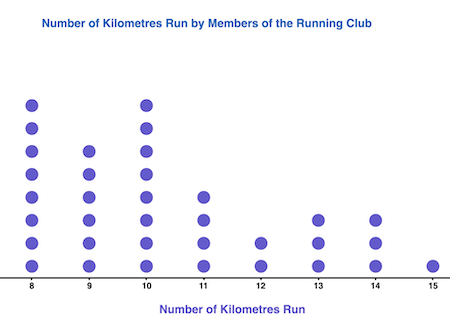
\includegraphics[width=0.75\textwidth]{dotplot.png}
    \caption{A dotplot showing the distribution of kilometers run by members of the running club.}
    \label{fig:dotplot}
\end{figure}

\emph{Dotplots} (as shown above) show each individual as a dot above their quantative data value.

When describing the shape of a dotplot (or other quantative graphs), \emph{focus on main features}: major peaks, clusters, or gaps. Especially note whether the distribution is roughly symmetric or skewed:

\begin{definition}[Symmetric, Skewed]
    A distribution is rougly \textbf{symmetric} if the right side of the graph has rougly the same shape as the left side.
    
    A distribution is \textbf{skewed to the right} if the right 'tail' has less values than the left; typically, the left has a peak whereas the right does not.
    \textbf{Left-skewed} definition are defined similarly to right-skewed distributions.
\end{definition}

For example, the distribution of the number of kilometers run is right-skewed because the right 'tail' has less values.

Graphs with a single peak are considered \emph{unimodal}, like the dotplot. Distributions with two peaks are considered \emph{bimodal}, and beyond that is considered \emph{multimodal.}

When describing a distribution of quantative data, use the acronym ROCS: \textbf{R}ange (max - min), \textbf{O}utliers (clear departures from the data), \textbf{C}enter (mean or median), and \textbf{S}hape (symmetry, skew, gaps, peaks).

Leaf plots exist. Stem represents first few digits, leaf represents final digit.

\begin{figure}[t]
    \centering
    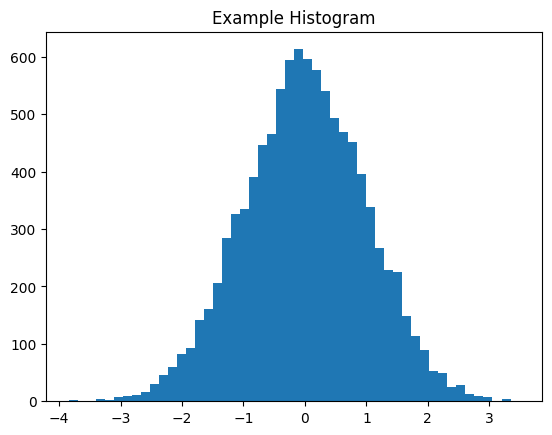
\includegraphics[width=0.75\textwidth]{histogram.png}
    \caption{An example histogram with a normal distribution.}
    \label{fig:histogram}
\end{figure}

\textbf{Histograms} are a notable way of displaying quantative data, as they avoid showing individual data points.
Histograms divide the variable into many 'bins' (bars), with the height representing the frequency. Smaller bins show more detail at the cost of a less clear pattern.

\textbf{Don't confuse histograms and bar graphs.} Histograms are used for quantative data, while bar graphs are used for qualatative data.

\textbf{Use percentages when comapring to distributions} in order to remove the effect of a larger sample.

\subsection{Describing Quantative Data with Numbers}
\begin{definition}[Mean: $\bar{x}, \mu$]
    The average of all individual data values. If there are \textit{n} observations $x_1, x_2, ..., x_n$, the sample mean is calculated by
    \[\bar{x} = \frac{\sum x_i}{n}\]
    The mean of a \textbf{sample} is referred to using $\bar{x}$, while the mean of a \textbf{population} is referred to using $\mu$.
\end{definition}

\textbf{Statistics} come from \textbf{samples} (small subset of population) and \textbf{parameters} come from \textbf{populations} (all possible samples of what's being tested).

The mean is not \textbf{resistant} as it is sensitive to strong outliers in a distribution. The median \textit{is} a resistant measure of the center of the distribution.

\begin{definition}[Median]
    The 'midpoint' of a distribution. Either the middle element ($n$ is odd) or the average of the two middle elements ($n$ is even) in a \textbf{SORTED} distribution.
\end{definition}

Using both the mean and the median, one can predict the skew of the data. If a distribution is rougly symmetric without outliers, \textbf{the mean and median will be similar}. If a distribution is strongly skewed, \textbf{the mean will be pulled in the direction of the skew}. (Mean $<$ Median for left-skewed, Mean $>$ Median for right-skewed)

The \textbf{range} (max - min) is one way to show the variability of a distribution. Note that the range is \textit{not} resistant.

\begin{definition}[Standard Deviation]
    The \textbf{standard deviation} ($s_x, \sigma$) measures the 'average' distance of the values in a distribution from the mean. Standard deviation is calculated by

    \[s_x = \sqrt{\frac{\sum{(x_i - \bar{x})^2}}{n - 1}}\]
\end{definition}

The squared stdev is known as \textbf{variance} ($s_x^2, \sigma^2$). Remember, $s_x$ refers to a sample while $\sigma$ refers to a population. Larger stdev indicates greater variation, but is not a resistant measure of variability. \textbf{Stdev measures variance around the mean; if the mean is skewed, so will stdev!}

The \textbf{Interquartile Range (IQR)} is another way to measure variance, using $IQR = Q_3 - Q_1$ where Q represents the quartiles. IQR can be thought of as the range of the 'middle half' of the distribution. \textit{IQR is a resistant measure.}

\[\textrm{Lower Outliers} < Q_1 - 1.5 \times IQR \textrm{ or High Outliers} > Q_3 + 1.5 \times IQR\]

boxplots and the five-number summary = min, Q1, median, Q3, and max exist. \textbf{Boxplots don't show gaps, clusters, or multiple peaks.}

be careful with language- 'skews' is a shape, IQR and range are single numbers (no 'in the middle of the IQR')

\newpage

\section{Modelling Distributions}
\subsection{Describing Location in a Distribution}
\begin{definition}[Percentile]
    The pth percentile of a distribution is the value with p\% of observations less than (\textit{or equal, depending on who you ask}) than it. Note that this distinction of whether or not to include "or equal" only matters for discrete variables.
\end{definition}

For example, in a class of 25 students, if a student gets a score greater than or equal to 21 other students, then they would be at the 84th percentile in the class's test score distribution ($\frac{21}{25} \approx 84\%$).
\textbf{An obervation is never "in" a percentile; an observation is AT a percentile} (percentile is just a number; like IQR and range). Also, definition, $Q_1 \approx 25$th percentile, $Q_2 \textrm{(median)} \approx 50$th percentile, and $Q_3 \approx 75$th percentile.
Percentiles can be graphically shown in a \textbf{cumulative relative frequency graph}, where the y-coordinates of points are graphed based on their percentile.

\begin{definition}[Standardized Score (z-score)]
    How many standard deviations an individual value is from the mean. For a value p, mean $\mu$, and stdev $\sigma$:
    \[z = \frac{p - \mu}{\sigma}\]
\end{definition}

z-scores provide a way to objectively compare measurements from two distributions while still considering means and variability.

\subsubsection{Transforming Data}

Effect of adding a constant a:
\begin{itemize}
    \item Adds a to measures of center and location (mean, median, quartiles, min, max)
    \item Does not change measures of variability (range, IQR, stdev)
    \item Does not change the shape of the distribution (percentile; translation along axis)
\end{itemize}

Effect of multiplying by constant b:
\begin{itemize}
    \item Multiplies measures of center and location by b (mean, median, quartiles, min, max)
    \item Multiplies measures of variability by $|b|$ (range, IQR, stdev)
    \item Does not change the \textit{overall} shape of the distribution (percentile; like squish or squash)
\end{itemize}

z-scores transform any distribution into one with mean 0 and stdev 1, but with the same original shape.

\subsection{Density Curves}
\begin{definition}[Density Curves]
    A curve that models the distribution of a quantative variable with a curve that
    \begin{itemize}
        \item Is always on (or above) the horizontal axis
        \item Has an area of exactly 1 underneath
    \end{itemize}
    The area under the curve within any interval of values estimates the proportion of all observations that fall into this interval.
\end{definition}

\textit{No set of quantative data is fully described by a density curve.} Density curves are approximations that are easy to use by smoothing out small irregularities in the data.
Similarly to finite distributions, distributions will have shapes, often with skews and peaks.

The median of the density curve splits the curve into two equal-area halves of area = 0.5.
The mean of the density curve is harder to define. For a density curve described by a function $p(x)$, the mean is given as the below.
(Intuitively, this is the idea of a 'weighted average'; weight being its relative density- $p(x)$, in this case- being extended to a continous distribution.)

\[\textrm{mean of $p(x)$} = \int_{-\infty}^{\infty}xp(x)dx\]
While the mean-median location principles still apply, they aren't too useful as it's relatively hard to locate the mean of a curve by simply looking at it.

\subsubsection{Normal Distributions}
As $\lim_{n\to\infty} n$, binomial distributions will approach a \textbf{Normal distribution} (see Chapter 6 or something), which are described using Normal curves.

\begin{definition}[Normal Curve]
    Any normal distribution is described by a symmetric, single-peaked, bell-shaped density curve. Its center is equal to the mean and the median, and the stdev represents the 'width' of the curve.
    Any normal distribution is fully described by its mean and stdev. A normal curve's mean is its peak, while the stdev are its inflection points (symmetric around the mean).

    Normal distributions with $\mu = 0$ and $\sigma = 1$ is known as a \textbf{standard Normal distribution} (which is the same as any other Normal distribution normalized into z-scores).
    \textit{Remember that mean and stdev only fully describe Normal distributions!}
\end{definition}

All normal distributions follow the \textbf{empirical rule}: 68\%, 95\%, and 99.7\% of all observations will fall within 1, 2, and 3 stdev around the mean respectively.
\verb|normalcdf(upper, lower, mean, stdev)| can be used to find the area under the normal curve (with a given mean and stdev) between upper and lower.
Similarly, \verb|invNorm(area to the left, mean, stdev)| calculates the area's percentile value given the mean and stdev.
\textbf{When using calculator functions like normalcdf, make sure to 1) label what the inputs mean and 2) answer the question asked AS A SENTENCE!}

\subsubsection{Assessing Normality}
uhh i'll do it later

\newpage

\section{Two-Variable Data}
\subsection{Scatterplots and Correlation}

When analyzing two sets of data, we usually hope to establish a cause-effect relationship between the \textbf{independent / explanatory variable} and the \textbf{dependent / response variable}.
We want to show that knowing the value of the independent value will help predict the dependent variable's value.
\textbf{Just because knowing the independent value helps us predict the dependent value does not imply direct causation; there may be some other variable influencing both!}

We can analyze two-variable using a scatterplot. To describe a scatterplot, consider the following:
\begin{itemize}
    \item \textbf{DIRECTION}: Does the dependent variable increase (\textit{positive assocation}) or decrease (\textit{negative association}) with the independent variable?
    Or does it look like there's no relation between the two? (\textit{no assocation})
    \item \textbf{FORM}: Is the data linear or nonlinear? Nonlinear data still shows a pattern, although it's harder to describe.
    \item \textbf{STRENGTH}: How closely does data follow the predicted pattern? Not very much (\textit{strong association}) or a lot (\textit{weak assocation})? Or somewhere between? (\textit{moderate association})
    \item \textbf{OUTLIERS}: Look at distinct departures from the described pattern and distinct clusters of points.
\end{itemize}

We can directly quantify correlation for linear relationships using the \textbf{(linear) correlation \textit{r}}.

\begin{definition}[Correlation \textit{r}]
    A measure of the direction and strength of a linear association.
    Always between -1 and 1, with values closer to each extreme indicating stronger relationships ($r = \pm 1 \rightarrow$ perfectly linear relationship, $r = 0 \rightarrow$ no linear relationship).
    Positive r suggests positive association, while negative r suggests negative association.

    \[r = \frac{1}{n - 1} \sum (\frac{x_i - \bar{x}}{s_x})(\frac{y_i - \bar{y}}{s_y}) = \frac{1}{n-1} \sum z_x z_y\]
\end{definition}

On a surface level, the formula for r standardizes each variable to avoid the issue of different linear slopes.
Other than that, don't ask why this formula works; it's wayyyy too much of a hassle to reasonably prove.

Obviously, r only works if both variables are quantative; use the word \textit{association} if either variables are categorical.
r doesn't differentiate between explanitory and response variables; r will be the same even if you swap the two sets.
r also has no units; it's just a scalar.

The linear correlation should only be used when talking about LINEAR relationships: a perfectly quadratic relationship will not give $r = 1$.
Linear correlation does not care about form; even if something is curved, linear correlation only measures its 'closeness' to a linear line.
\textbf{Linear correlation is not resistant; it is GREATLY influenced by extreme points.}

\subsection{Least-Squares Regression}

\begin{definition}[Regression Line]
    A line of form $\hat{y} = a + bx$ which models how the dependent variable y changes as the independent x changes.
    ($\hat{y}$ = predicted value of y for given x)
    \textbf{Regression lines require that we consider the x as the independent variable.}
\end{definition}

Alternatively, we can think of $\hat{y}$ as the average price for a sample of individuals with the same x value (assuming that our pattern is true).
Beware of \textbf{extrapolation}: using a regression line to predict outside of the interval of x-values used to obtain the line.
The further the values are from the data used to generate the line, the less reliable the prediction is.
\textit{Just because regression lines can predict extreme values doesn't mean those values will ever happen!}

\subsubsection{Residuals}
To determine if a regression line is a good prediction, plot the \textbf{residuals} ($y - \hat{y}$ for all data points in the set).
No pattern suggests that the regresison model is accurate, while a leftover non-zero pattern suggests that this model isn't appropriate. (Close to the x-axis = strength)

Intuitively, we look at the remaining pattern because \textbf{form of residual plot = form of association - form of model}.
As ssuch, no residual plot form suggests that form of association = form of model (good), while a residual plot form suggests that form of assocation $\neq$ form of model (bad!!!).

\subsubsection{Least-Square Regression Lines}

A good regression line minimizes the \textbf{sum of the squared residuals.} (Why not the residuals themselves? The sum of all the residuals = 0, so we square it to avoid sign- similar to stdev.)
The line that minimizes the squared residuals is known as the \textbf{least squares regression line}.

The least-square regression line $\hat{y} = a + bx$ can be calculated as follows:

\[b = r\frac{s_y}{s_x}\]
\[a = \bar{y} - b \bar{x}\]

The formula for the slope can be thought of as "normalizing" the correlation to fit with the specific scenario using the coefficent $\frac{s_y}{s_x}$.
(as far as i can tell there's no super intuitive way to think about this. sorry)

The formula for the y-intercept comes from the fact the least-squares regression line will always pass through $(\bar{x}, \bar{y})$. Using simple algebra we re-arrange for a.

This is called \textit{regression to the mean} because something something predicted values "regress" to the mean somehow.

\subsubsection{Problems with Least-Square Regression Lines}
Similar to correlation, least-square regression lines are 1) only used to describe linear relationships, 2) not resistant, and 3) only describe patterns in the data, not direct causation.

2 suggests that points with relatively high or low x-values have \textbf{high leverage} over the regression line versus other points in the data set.
These \textbf{outliers} (original def + high residual) are \textbf{influential points}; if removed, they substantially change the regression line or measures of strength (see 3.2.4).


\subsubsection{Strength of regression lines}

To determine the strength of a regression line, we have two methods: the \textbf{standard deviation of the residuals} or the \textbf{coefficent of determination $r^2$}.

The standard deviation of the residuals ($s$) is pretty obvious: calculate the stdev of the data relative to the prediction. (why n - 2? idk it looks rlly complicated)
\[s = \sqrt{\frac{\sum (y_i - \hat{y}_i)}{n - 2}}\]

On the other hand, the coefficent of determination measures the percent reduction in the sum of squared residuals when using the regression line vs. using $\hat{y} = \bar{y}$.
In other words, it represents the percent of variability in the response variable that is accounted for by the least squares regression line.
($1 - r^2$ can be thought of as the \% of variability that's caused by other factors than the independent variable.)
(It's also equal to the square of the linear correlation, hence the symbol $r^2$. why? idk)

\[r^2 = \frac{\sum (y_i - \bar{y})^2 - \sum (y_i - \hat{y})^2}{\sum (y_i - \bar{y})^2}\]

\subsection{Transforming to Achieve Linearity}

The techniques discussed in 3.1 and 3.2 (obviously) only apply to purely linear relationships.
In some special cases, we may be able to \textbf{tranform the data} from a non-linear pattern into a linear pattern to apply our techniques.

\subsubsection{Power Models}
\begin{definition}[Power Model]
    Any regression model that takes the form $\hat{y} = ax^p$.
    Scenarios modeled by these regression models should be expected to do so by geometry (eg. area proportional to square, volume proportional to cube) or some other factor like physics.
\end{definition}

While power models (by definition) describe a non-linear relationship between x and y, there will always be a linear relationship between $x^p$ and y.
As such, if we raise x to the pth power or take the pth root of y there should be a linear relationship between $x^p$ and y (or x and $\sqrt[p]{y}$).

However, this all assumes p is known. If p isn't known, you could either guess and check (cringe) or use logarithms.

\subsubsection{Transforming with Logarithms}

If a scenario is modeled by $y = ax^p$, then $\ln(y) = \ln(ax^p) \rightarrow \ln(y) = \ln(a) + p\ln(x)$.
Thus, there is a linear relationship between $\ln(x)$ and $\ln(y)$.
(\textit{Note that the power p now becomes the slope of the line!})
If the resulting graph turns out ot be linear, we can fit a linear regression line to the graph and then use the relation $\hat{y} = e^{a + b\ln(x)}$ to predict values.
(This relationship is the same as the power model: $\hat{y} = e^a \times e^{b\ln(x)} = e^a x^b$; $e^a$ is a constant.)

If a scenario is modeled by $y = ab^x$ (an \textbf{exponential model}), then $\ln(y) = \ln(ab^x) \rightarrow \ln(y) = \ln(a) + \ln(b)x$.
Thus, there is a linear relationship between x and $\ln(y)$.
IF the resulting graph turns out to be linear, we can fit a linear regression line to the graph and use the relation $\hat{y} = e^{a + bx}$.
(This relationship is the same as the exponential model: $\hat{y} = e^a \times e^{bx} = e^a \times (e^b)^x$: $e^a$ and $e^b$ are constants.)

If unsure if an exponential or power model is better, consider their residual plots.
If both models have similarly random residual plots, choose the model with the largest $r^2$.


\newpage

\section{Collecting Data}
most yap based chapter. almost no math :/

\subsection{Sampling and Surveys}

In statistics, we often want to discover things about a large group of people (the \textbf{population}).
While we could survey \textit{everybody} in a \textbf{census}, this is often incredibly impractical for obvious reasons.
Instead, we often consider only a small \textbf{sample} (subset) of people to represent the population, in a \textbf{sample survey} (a study of a sample to predict things about the population).
From the data we observe in the sample, we can make predictions about the population as a whole.
\textit{Surveys include but aren't restricted to just questions.} They can include asking people to do something, and observing how they go around doing it.

\subsubsection{What is Bias?}
\begin{definition}[Bias]
    The design shows bias if it is very likely to underestimate or overestimate the value you're trying to predict.
    (Remember, the statistical analyses discussed in Chapters 8-12 don't consider bias!)
\end{definition}

\textbf{Bias is not bad luck in one sample}- Bias will consistently miss the truth in the same way.
When asked to describe how a statistical study shows bias:
\begin{itemize}
    \item Describe how members of the sample might respond differently vs. the population
    \item Explain how this difference might lead to an overestimate or underestimate
    \item \textbf{Don't overthink it}- it should be a "common sense" explanation.
\end{itemize}

\subsubsection{Sources of Bias}

\begin{definition}[Convenience Sampling]
    Selecting individuals from a population that are easy to reach.
    May cause bias due to nearby individuals sharing some characteristics (like a club or class)
    Eg. asking about sports in a library.
\end{definition}

\begin{definition}[Voluntary Response Sampling]
    Allowing people to \textit{choose} whether or not they are part of a sample.
    Often causes bias due to attracting people who feel strongly about an issue, share some common opinion, or who are more confident.
\end{definition}

\begin{definition}[Undercoverage]
    When some members of a population are less likely or unable to be chosen in a sample.
    Eg. selecting a sample from a list of houses ignores dormitory students, homeless people, and prisoners.
\end{definition}

\begin{definition}[Nonresponse]
    When an individual chosen for the sample can't participate (voluntary or involuntary).
    May lead to bias as those who don't respond may respond differently vs. those who do participate.
    Eg. landline calling people to ask if they go on runs- people unable to pick up may be on a run and thus run more.
\end{definition}

\begin{definition}[Response Bias]
    A systematic pattern of inaccurate answers to a survey question.
    Often due to \textbf{question wording bias}: the wording of the question causes some confusion or leads individual to one specific conclusion.
\end{definition}

\textbf{Voluntary response does not explain why certain people don't respond in an individual survey.}
Nonresponse can only happen after a sample has been selected.
In a voluntary response sample, every individual has \textit{opted} to take part, so there won't be any nonresponse.

\subsubsection{How to Avoid Bias}
\begin{definition}[Random Sampling]
    Using some sort of chance process to determine which members of a population are included in a sample.
    \textbf{Chance process specifically- not just "arbitrary!"}
\end{definition}

\begin{definition}[Simple Random Sample (SRS)]
    A sample size n selected by random sampling such that every group of n individuals in a population has a equal chance of being selected as part of the sample.
    Should be done using \textbf{sampling without replacement.}

    When using technology: label all people in the population 1... N, use a rng to generate n \textit{different} integers 1-N, then use the people corresponding to the rng.
    When using a table, \textbf{make sure to choose a system s.t. every number has an equal chance of occuring!}
\end{definition}

\begin{definition}[Sampling with(out) replacement]
    An individual from a population may only be selected once (without replacement) or multiple times (with replacement).
\end{definition}

\begin{definition}[Stratified Random Sampling]
    Dividing a populations into groups that share certain characteristics (\textbf{strata}), selecting SRSes from the strata, then combining them into one random sample.
    Yield more accurate results \textbf{IF} individuals within each strata are \textbf{homogenous} (similar).
\end{definition}

\begin{definition}[Cluster Sampling]
    Dividing a population into groups in the population into non-overlapping groups (\textbf{clusters}) that \textit{don't} share common characteristics, picking some clusters, and then combining them into one random sample.
    Less accurate than stratification, but obviously more practical- much easier to access clusters vs. strata.
    Yields more accurate results \textbf{IF} individuals within each strata are \textbf{heterogenous} (different).
\end{definition}

\begin{definition}[Systematic Random Sampling]
    Selecting a sample from an ordered arrangement of the population by randomly selecting one of the first k individuals, then picking every kth individual after for a sample.
    Very useful for continous streams of people, where the number of people isn't known before hand; eg. voting booths.
    \textbf{If there are patterns in the way the population is ordered that coincide with the pattern being chosen, then the sample likely isn't representative of the population.}
    (Eg. some people are late, take up more of the sample)
\end{definition}

\subsection{Experiments}
Surveys are one kind of \textbf{observational studies}: studies that observe individuals and measures variables of interest, but does not attempt to influence the responses.
Split into \textit{retrospective} (look at the past) and \textit{prospective} (look into the future).
Prospective studies are more useful than retrospective studies, as other influences on certain variables are much easier to track.

\begin{definition}[Experiment]
    Deliberately imposes conditions (\textbf{treatments}) on \textbf{experimental units} (the object the treatment is being applied to: if human, use \textbf{subjects}) to measure their responses.
    Treatments are sometimes known as \textbf{factors}; \textbf{explanatory variables} whose different \textbf{levels} may cause different changes in the \textbf{response variable}.
    Surveys show correlation between two variables exist, expeirments show cause and effect between two variables.
\end{definition}

Experiments should be designed to avoid \textbf{confounding}: two or more variables can be shown to possibly be an independent variable without direct conformation (better definition?).
One notable type of confounding to consider is the \textbf{placebo effect}: some subjects will genuinely improve because they think they will, not due to the treatment.
To counteract this, one treatment should typically be a \textbf{control group}; a group not given treatment (whether completely no treatment or fake treatment) in order to compare whether the treatment causes some change.

\textit{The placebo effect also applies to the experiment designers, too!}
Experiments should ideally be \textbf{double blind} (neither the subject nor the interviewer knows what treatment the patient is recieving).
Obviously, this might not be possible for some experiments.
For this case, experiments should still attempt to be \textbf{single blind} (either the subjects or the intervewers don't know which treatment a patient is recieving).

There are two discussed types of experiment designs: \textbf{Completely Randomized Design}, where experimental units are assigned to treatments completely at random, and \textbf{Randomized Block Design}, where experimental units are divided into similar groups (\textbf{blocks}; like strata) and then tested using completely randomized testing individually.
\textbf{Matched Pair design} is one specific type of experimental design for comparing treatments of block size 2.
Typically, two very similar experimental units (some type of pair) are made into a block and are given the treatment randomly.

\subsubsection{Principles of Experimental Design}
\begin{itemize}
    \item \textbf{Comparison}: use a design that compares two or more treatments (at least a Control Group)
    \item \textbf{Random Assignment}: use a chance process to assign experimental units avoids confounding
    \item \textbf{Control}: keep other variables same for all groups, especially other counfounders
    \item \textbf{Replication}: more sample size = less likely varation in the effects is due to random chance
\end{itemize}

\subsection{Using Studies Wisely}

Obviously, a sample isn't a population, so there's going to be some varation in the data you observe in the sample versus the population.
This is knwon as \textbf{sampling variability}.
Bigger sample size = less variability. Duh.

When the observed results of a study are too unusual to be explained by chance alone, the results are \textbf{statistically significant.}
\textit{Statistical significance does not account for bias!}

When inferring from data, keep in mind \textbf{what population individuals come from}, and \textbf{random assignment to groups allows inference on cause and effect}.
Observational studies should \textbf{almost} never be used to demonstrate cause and effect. Unless:
\begin{itemize}
    \item Association ($R^2$?) is very strong
    \item Association is consistent (does not vary between different populations)
    \item Larger values of explanitory = stronger response (stopping = lese response)
    \item Cause always preceeds effect in time (not something else)
    \item Alleged cause makes intuitive sense (or has some other history that makes it plausible)
\end{itemize}

\subsubsection{Data Ethics*}
i'm not doin allat

\newpage

\section{Probability}

\newpage

\section{Random Variables and Distributions}

\newpage

\section{Sampling Distributions}

\newpage

\section{Confidence Intervals}

\newpage

\section{Significance Tests}
\textbf{Significance Tests} are like the opposite of confidence intervals. Instead of using a statistic to find a parameter, significance tests use statistics to test claims about a parameter.

\begin{definition}[Significance Test]
    A formal procedure for using observed statistics in order to decide between to competing claims (\textit{hypotheses}) about parameters.
\end{definition}

\subsection{Basics of Significance Tests}
\subsubsection{Hypotheses}
\begin{definition}[Null Hypothesis, $H_0$]
    A claim about a parameter that we weigh evidence \textbf{against} in a significance test. Usually a statement of 'no difference' (as claimed).
\end{definition}

\begin{definition}[Alternative Hypothesis, $H_a$]
    The claim that we are trying to find evidence for. Directly contradicts the null hypothesis.
\end{definition}

This "Null Hypothesis" and "Alternative Hypothesis" can be thought as trying to prove someone "guilty" or "not guilty."

For example, if a player claims they're a 80\% free throw player, the null hypothesis would be $H_0: p = 0.80$, and the alternative hypothesis would be $H_a: p < 0.80$.

The alternative hypothesis is \textbf{one-sided} because we suspect that the player makes less than 80\% of his free throws. If we believe that it's equally plausible that they make more than 80\% of their free throws, then we would use a \textbf{two-sided hypothesis}- $H_a: p \neq 0.80$.

\textbf{Hypotheses express our beliefs before looking at the data}. Molding a hypothesis around data shows nothing.
(11.1) \textbf{Just because a test is statistically significant does NOT mean that it is PRACTICALLY significant.}
Focus on the P-value and better yet, the data itself.
Graph your data and see if differences or outliers are significant, or if there's another pattern emerging.
Generally, for practical importance, it's much better to give a confidence interval versus a significance test.

\subsubsection{P-values}
\begin{definition}[P-value]
    The probability of getting the values observed in the data under the assumption that the null hypothesis $H_0$ is true.
\end{definition}

Small P-values provide convincing evidence for the alternative hypothesis because small values suggest the observed result is unlikely to happen when the null hypothesis is true.
Similarly, large P-values provide convincing evidence for the null hypothesis because large values suggest the observed result is likely to happen due to chance if the null hypothesis is true.

In terms of probability notation: P-value = P(observed data $|$ null hypothesis is true).

For two-sided tests, we look at the distance between the null hypothesis and the observed data.
For example, if $H_0: p = 0.5$, $H_a: p \neq 0.5$ and $\hat{p} = 0.65$ (observed proportion), then the P-value = P($\hat{p} \leq 0.35$ or $\hat{p} \geq 0.6$ $|$  $p = 0.5$).
We look at $\hat{p} \leq 0.35$ because $|p - 0.35| = |p - 0.65|$.

Based on the P-value, we make a conclusion about data:
\begin{itemize}
    \item If the P-value is small (unlikely to happen by chance), then we "reject $H_0$" and conclude that there is convincing evidence for $H_a$ (in context).
    \item If the P-value is large (likely to happen by chance), then we "fail to reject $H_0$" and conclude that there is not convincing evidence for $H_a$ (in context).
\end{itemize}

How small does a P-value have to be in order to reject $H_0$? We use a given \textbf{significance value} for this boundary.

\begin{definition}[Significance Level, $\alpha$]
    The value that we use as a boundary for deciding whether a P-value is significant enough to disqualify the null hypothesis. \textit{$\alpha$ should be stated before data is produced (cherrypicking).}
    \[\textrm{P-value} < \alpha \Rightarrow \textrm{reject } H_0\ \Rightarrow \textrm{convincing evidence for $H_a$ in context}\]
    \[\textrm{P-value} > \alpha \Rightarrow \textrm{fail to reject } H_0\ \Rightarrow \textrm{not convincing evidence for $H_a$ in context}\]
\end{definition}

If P is less than the significance level, we say that the result is "statistically significant at the $\alpha = \_\_\_\_$ level."
Alternatively, "the results were significant ($P = 0.03 < \alpha = 0.05$)."
\textit{Keep in mind a P-value is more informative than a statement of significance!}

\textbf{NEVER "accept $H_0$" or conclude that $H_0$ is true!} Always use 'reject' or 'fail to reject!'

(11.1) \textbf{Beware of multiple analyses.} A signifiance test of $\alpha = 0.05$ is reasonable enough to prove something on its own.
But if you take 20 tests of $\alpha = 0.05$ and record if any of them show your conclusion- well, that doesn't really show anything! "Searching for patterns is fine. But performing every conceivable significance test on a data set until you obtain a statistically significant result is not."
(This is known as \textit{P-hacking or data dredging.})

\subsubsection{Type I and Type II Errors}
When drawing a conclusion from a significance test, our conflusion may be wrong.
There are two types we can make with the conclusion process, helpfully named "Type I" and "Type II" errors. Only one type of error is possible at once.

\begin{definition}[Type I and II errors]
    A \textbf{Type I error} occurs when we reject $H_0$ when $H_0$ is true; the data gives convincing evidence that $H_a$ is true despite being false.
    
    A \textbf{Type II error} occurs when we fail to reject $H_0$ when $H_a$ is true; the data fails to give convincing evidence that $H_a$ is true despite it being true.
\end{definition}

Note $P(\textrm{Type I error}) = \alpha$.
However, significance is inversely proportional to Type II error: as significance decreases, $P(\textrm{Type II error})$ increases.

\subsubsection{Power}
\begin{definition}[Power]
    The \textbf{power} of a test is the probability that the test finds convincing evidence for $H_a$ given that the parameter is a specific value that does follow $H_a$. In other words:
    \[\textrm{power} = P(\textrm{reject $H_0$ $|$ $H_0$ is false})\]
\end{definition}

\textit{Power depends on a specific value.} For example, if the power of a test to detect p = 0.08 is 0.29 given $H_0: p = 0.10$, if the true proportion in the population is p = 0.08, there is a 0.29 probability that researchers will find convincing evidence for $H_a$.

Note Power = 1 - P(Type II Error), or written alternatively, P(Type II Error) = 1 - Power. Also note that the power of a test increases with higher sample number, higher signifiance level, further null and alternative parameter values, and 'wise choices when collecting data' (reducing variability).
\textit{Larger signifiance values reduce the chance for Type II error, but increase the chance for Type I error.}

\subsubsection{Steps for Signifiance Tests}
Overall, significance tests can be summarized in four steps:
\begin{enumerate}
    \item \textbf{STATE} the hypotheses, signifiance level, and parameters.
    \item \textbf{PLAN} the appropriate inference method and check conditions.
    \item \textbf{DO} the signifiance test (see Section 7.2): \begin{itemize}
        \item Give the sample statistic(s)
        \item Calculate the standardized test statistic
        \item Find the P-value.
    \end{itemize}
    \item \textbf{CONCLUDE} whether or not you believe in the null or alternate hypotheses, with reference to P-values, in the context of the problem. Make sure to reference the parameter, not the sample statistic!
\end{enumerate}

\subsection{Tests About a Population Proportion}

Like confidence intervals, signfiicance tests should satisfy several conditions; random sampling, no bias, 10\% if applicable ($n < 0.10N$), and large counts ($np_0 \geq 10$ and $n(1-p_0) \geq 10$).
Note that the large counts condition uses $p_0$: the number of successes and failures \textit{assuming the null hypothesis is true} are both greater than or equal to 10.

To conduct a \textbf{one-sample z test for a proportion} (CITE THIS WHEN FOLLOWING THE SIGNIFIANCE TEST STEPS) about a proportion, look at the normal distribution \textit{assuming the null hypothesis is true.}

From Section 7.2 (add ref later), $\mu_{\hat{p}} = p_0$ and $\sigma_{\hat{p}} = \sqrt{\frac{p_0(1-p_0)}{n}}$.

Using this, we standardize the statistic with respect to the null value to get the \textbf{standardized test statistic}; how many stdev units away the sample statistic is from what we would expect, assuming the null hypothesis is true.
\textbf{YOU HAVE TO PUT THE STANDARDIZED TEST STATISTIC ON THE TEST!}

\[\textrm{standardized test statistic} = z_{sts} = \frac{\hat{p} - \mu_{\hat{p}}}{\sigma_{\hat{p}}}\]

Using this, we can directly find the P-value using \verb|normalcdf| with the appropriate values:
\begin{itemize}
    \item $P(z > z_{sts})$ if $H_a : p > p_0$
    \item $P(z < z_{sts})$ if $H_a : p < p_0$
    \item $P(z > |z_{sts}|) + P(z < -|z_{sts}|)$ if $H_a : p \neq p_0$
\end{itemize}

Keep in mind that just because the P-value is low \textit{does not prove that $H_0$ is false}; sample proportions may be small due to sampling variability, or we have made a Type I error somehow. \textbf{AVOID JUMPING TO CONCLUSIONS}: just because a sample statistic looks unlikely, doesn't mean its P-value is!

It should be noted there is a link between \textit{two-sided tests} and confidence intervals: a K\% confidence interval gives an approximate set of $p_0$'s that would not be rejected by a two-sided test at the $\alpha = \frac{K}{100}$ level, with all other values being rejected.

Intuitively, if a confidence interval for p using \textit{the same} $\hat{p}$ does not include $p_0$, as the distribution (test) about $p_0$ has a similar stdev (due to the same $\alpha$) the distribution is unlikely to include the actual value of $p$.

\subsection{Tests About a Difference in Proportions}
Tests about difference in proportions work very similarly to tests about single proportions. For null hypothesis $H_0 : p_1 - p_2 = 0$, large counts can't directly be applied; we need estimate the true difference in proportions p using a weighted average of the two proportions:

\[\hat{p}_C = \frac{\textrm{number of successes in both samples combined}}{\textrm{number of individuals in both samples combined}} = \frac{n_1 \hat{p}_1 + n_2 \hat{p}_2}{n_1 + n_2}\]

We use this pooled proportion (\textit{even for non-zero differences}, although the given formulas have to be changed) because the combined proportion provides \textit{the best estimation of the true difference in proportions}.
In the one-sample z test for a proportion, we used $p_0$ because we're looking at the distribution relative to it.
For \textbf{two-sample z tests for the difference between two proportions}, we look at the distribution 'relative' to the true proportion; which our best guess is $\hat{p}_C$.
(something something using each individual $\hat{p}_i$ causes too much error + causes some error in the underlying math when we're testing for 0 diff)

In this case, we use the combined proportion for large counts \textit{for both samples}: that is, $n_1 \hat{p}_C, n_1 (1 - \hat{p}_C), n_2 \hat{p}_C, n_2 (1 - \hat{p}_C)$ all need to be greater or equal than 10.
Using the combined proportion works for a non-zero difference in the null hypothesis, although is not strictly neccessary (large counts for each individual distribution can be used).

The standardized test statistic also uses the combined estimate (for both proportions are equal; otherwise, each individual statistic can be used):

\[z = \frac{(\hat{p}_1 - \hat{p}_2) - 0}{\sqrt{\frac{\hat{p}_C (1 - \hat{p}_C)}{n_1} + \frac{\hat{p}_C (1 - \hat{p}_C)}{n_2}}}\]

\newpage

\section{Estimating Means}

\subsection{One-Sample \textit{t} intervals}

To create a confidence interval for a mean, we can use the same point estimate $\pm$ margin of error = (critical value)(SE of statistic) idea.
However, this is slightly flipped, as (from Section 7) the stdev of a sample distribution relies on the stdev of the population itself.
If we know the stdev of the population, we can the familiar \textit{one-sample z interval for a population interval}:

\[\hat{\mu} = \bar{x} \pm z^{*}\frac{\sigma}{\sqrt{n}}\]

\textit{Using the sample stdev alone is not a good enough approximation}.
For an example, using the sample stdev to estimate a 99\% confidence interval would result in a $\approx 92.5\%$ confidence interval.
This is because there is significant variation in the sample stdev itself.

To account for this, we use the larger \textit{t-distribution} instead.
The t-distribution is like the z-distribution (measures how many stdevs needed for desired confidence), but has higher area in the tails to compensate for the errors in the sample stdev.
Notably, t-distributions vary depending on the sample size; that is, they have a specific \textit{degree of freedom df.}
(Use \verb|invT| to calculate the specific $t^{*}$ value needed.)
When using t-distributions, make sure to set $df = n - 1$. Thus, for the \textit{the one-sample t interval for a population mean,}

\[\hat{\mu} = \bar{x} \pm t^{*}\frac{s_x}{\sqrt{n}}\]

The random (and 10\%) clauses still apply, although the Large Counts condition is slightly modified due to the central limit theorem:
\begin{itemize}
    \item If the sample size is small ($n < 30$), then graph the sample data (dotplot is preferred, although boxplot works it's kinda funky) and consider whether the data plausibly comes from a normal population.
    No strong outliers or skew indicates yes. \textit{You will have to show your graph when assesing the normality of the data.}
    \item If the sample size is big ($n \geq 30$), then you can still use a one-sample t interval for a population mean (although the true confidence level will be lower than presented).
\end{itemize}

The \verb|TInterval| function on the calculator can be used to simulate a one-sample t interval for a population mean if the above are satisfied.

\textit{As $df \rightarrow \infty$, the t-distribution approaches the normal distribution.}
Intuitively, as sample size increases, the sample stdev will get closer to the population stdev.
The quantity $\frac{s_x}{\sqrt{n}}$ is known as the \textit{standard error of the sample mean} ($s_{\bar{x}}$).

\subsection{Two-Sample \textit{t} intvervals for a Difference between Two Means}

Like two-sample z intervals, these require the one-sample requirements to be fufilled for the populations, and follow the same idea (sqrt the variance):

\[\hat{\mu}_{x_1 - x_2} = (\bar{x_1} - \bar{x_2}) \pm t^{*}\sqrt{\frac{s_1^2}{n_1}+\frac{s_2^2}{n_2}}\]

However, the degrees of freedom are significantly more confusing to decide. There are two practical options to decide the df to use:
\begin{itemize}
    \item \textbf{Technology}: Use the formula below to calculate df. Note that in this case, df is usually not a whole number.
    Results in confidence intervals that are approximately the stated confidence levels.
    \[df = \frac{{(\frac{s_1^2}{n_1} + \frac{s_2^2}{n_2})}^2}{\frac{1}{n_1 - 1} {(\frac{s_1^2}{n_1})}^2 + \frac{1}{n_2 - 1} {(\frac{s_2^2}{n_2})}^2}\] % touch this and die

    \item \textbf{Conservative}: $df = \min{(n_1 - 1, n_2 - 1)}$.
    Note this method causes a margin of error as large if not larger than is needed for the desired confidence level.
\end{itemize}

\subsection{Paired \textit{t} interval For a Mean Difference}
(also known as a one-sample t inerval for a mean difference)

For comparing data which interviews the "same" (or highly related) individuals (known as \textbf{paired data}), "combine" the data into one dataset by subtracting each individuals' values, and analyze that using the tactics from section 10.1.
(n = the number of pairs)

The requirements are the same as the 1-sample t interval, although the meaning of 10\% ($n_{diff} < 0.10N_{diff}$) is different: we suspect that the data is not independent, so 10\% guarantees that the differences are independent.





\newpage

\section{Confidence with Means}
tl;dr the same thing as Section 9 but with means this time (it works how you think it does)
\subsection{Tests about a Population Mean}
Null hypotheses, alternative hypotheses, and significance levels exist and mean the same thing as they did in Section 9. Yipee!

While the random and 10\% conditions still apply, the large counts condition is modified to account for the Central Limit Theorem, like described in Section 10.1.
To reiterate; if the $n < 30$, check whether the data is approximately Normal (no major skew or outliers) before performing tests; otherwise, everything proceeds as normal (haha).
Dotplots are reccomended to check for Normality due to ease, but other graphs work too.

As before, we need to calculate a standardized test statistic and a P-value.

\[\textrm{standardized test statistic} = z = \frac{\bar{x} - \mu_0}{\sigma_{\bar{x}}} = \frac{\bar{x} - \mu_0}{\frac{\sigma}{\sqrt{n}}}\]

Obviously, $\sigma$ for the population is rarely known. So we use the \textit{standard error of $\bar{x}$} once again:

\[t = \frac{\bar{x} - \mu_0}{\frac{s_x}{\sqrt{n}}}\]

Instead of using the Normal distribution (like you would when $\sigma$ is known), you will need to use a \textit{t-distribution}, like Section 10 describes.
Same \verb|tcdf|, $df = n - 1$, etc.
Remember, if you're lazy: $P(t \geq k) = P(t \leq -k)$ for both Normal and t distributions. No calculator for t-distribution? Use the tables, but be wary to give a range between the floor and ceil of the df.

The same link between two-sided confidence intervals and confidence intervals exist.
Interestingly, there's also a relation between one-sided tests and confidence intervals for a population mean.- a one sided test is the same as a confidence interval with $C = 1 - 2\alpha$.

Difference in means and paired means work exactly like you think they do.
Remember to use $\bar{x}_{diff}$ and $s_{diff}$ for paired data.
Remember to use $df = min(n_1 - 1, n_2 - 1)$ or technology; don't use the sum.

(idk put this somewhere else) \textbf{Use one-sample t procedures when testing data collected in pairs. Use two-sample difference t procedures when testing data collected from two populations independently.}
\newpage

\section{Inference for Distributions and Relationships}

\subsection{Chi-Square Tests for Goodness of Fit}
Obviously, the significance tests and confidence intervals discussed in sections 7 - 11 only apply to single continous variables.
This obviously raises the question: \textit{what if you want to consider multiple variables at once?}

Say, for example, several mutually exclusive proportions, like dice rolls.
Of course, you could run a single-variable test on every single sample proportion to see if it matches up with what you expect.

Besides the obvious problem of being fairly inefficent, this also raises the problem of multiple tests indirectly leading to \textbf{P-hacking} (running several tests until you get a statistically significant result).
Additionally, it doesn't tell you how likely it is to get a random sample with the given sample distribution assuming the claimed proportions are true.
Instead, we need to consider all proportions at once, using a \textit{chi-square test for goodness of fit.}

For our null hypothesis, we assume that the claimed distribution is true.
This leads to the obvious alternate hypothesis: the true distribution is not the same the claimed distribution.
For example, dice rolls:
\begin{itemize}
    \item $H_0$: The distribution of dice rolls is the same as the claimed distribution.
    In other words: $p_i = \frac{1}{6}$ where $p_i$ represents the proportion of dice rolls that land ith side up.
    \item $H_a$: The distribution of dice rolls is not the same as the claimed distribution.
    At least two of these proportions differ than the values stated in the null hypothesis (2 cause $\sum p_i = 1$) 
\end{itemize}

Like other significance tests, we compare our \textit{expected values} (assuming the null hypothesis is true) to our experimental data.
Say we roll a dice 60 times. Then, our expected count for categorical variable i in the distribution is $np_i = (60)(\frac{1}{6}) = 10$ rolls to come up for each side of the die.
($np_i$ \textit{may not be an integer, and shouldn't be rounded to one.})

To quantify how far our experimental data is compared to our expected data, we calculate the \textit{chi-square test statistic}.

\begin{definition}[Chi-square test statistic, $\chi^2$]
    A measure of how far each experimental count differs from the expected count for each categorical variable. (Summed over all possible values for the categorical variable, \textit{k}.)
    \[\chi^2 = \sum \frac{(\textrm{Observed Count} - \textrm{Expected Count})^2}{\textrm{Expected Count}} 
                = \sum_{i=0}^{k} \frac{(n\hat{p_i} - np_i)^2}{np_i}\]
\end{definition}

Make sure to use the COUNTS, and not the PROPORTIONS when calculating $\chi^2$.
We square the difference for similar reasons to $\sigma$: to get rid of sign (i think).
We divide by the expected count to encode its relative significance, instead of prioritizing extremely high differences.

\begin{figure}[t]
    \centering
    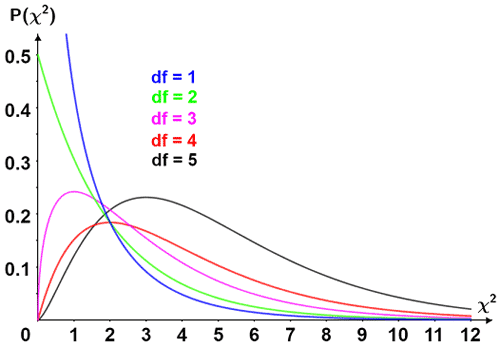
\includegraphics[width=0.75\textwidth]{chi-square-distribution.png}
    \caption{A probability density plot showing chi-square distributions with $df = 1, 2, 3, 4, 5$.}
    \label{fig:chi-square-dist}
\end{figure}

Similar to previous significance tests, we look at the \textit{chi-square distribution} to generate a P-value.
Chi-square distributions are right-skewed non-negative distributions (due to the square) that also take in degrees of freedom (df) = number of categorical variables - 1.
The mean of a chi-squared distribution is equal to df and has a singular peak at df - 2 (df $>$ 2).

Similar to previous significance tests, the random and 10\% conditions still apply.
Large counts is slightly modified; all \textit{expected} counts should at least be 5.

Use the chi-squared cdf function on your calculator to generate a P-value.
(\textit{Remember, your P-value is the area to the RIGHT of your $\chi^2$ value; your lower value should be your test statistic, not the upper!})
From there, use the stated significance level to either reject or fail to reject the null hypothesis.
\textit{Remember that just because we fail to reject the null hypothesis does NOT mean that it is true.}
We simply don't have data to reject the null hypothesis.

If you are asked how the distribution is different than the predicted distribution, note which categories that contribute the most to $\chi^2$.
Then, describe how the observed and predicted counts for these categories differ, with reference to direction. (less or more?)

\subsection{Inference for Two-Way Tables}
\begin{figure}[t]
    \centering
    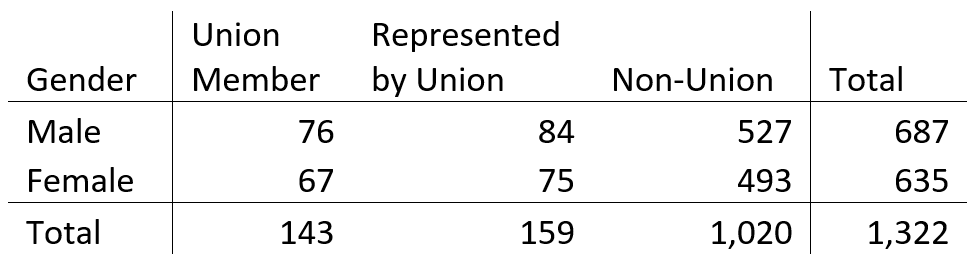
\includegraphics[width=0.75\textwidth]{chi-square-homogenity.png}
    \caption{A two-way table comparing gender and union participation.}
    \label{fig:chi-square-homo}
\end{figure}

Two-sample z tests (discussed in section 9.3) allow us to compare proportions in two populations or two treatments.
\textit{Chi-square tests for homogenity} allow us to compare distributions of a single categorical variable across several populations or treatments.
\textit{Chi-square tests for independence} allow us to analyze whether there's evidence of an association between two variables.

\subsubsection{Chi-square tests for homogenity}
To begin, create a two-way table like shown in Figure \ref{fig:chi-square-homo}.
Generally, our null hypothesis says that there is \textit{no difference} in the true distribution of a categorical variable in the populations of interest (or treatments in an experiment).
In this case, our null hypothesis would be $H_0$: There is no difference in the true distributions of union participation if the worker is male or female.
Similarly, the alternate hypothesis says that \textit{there is a difference, but does not specify what that difference is.} ($H_a$ works for ANY difference in distribution.)
In this case, $H_a$: There is a difference in the true distributions of union participation if the worker is male or female.

(doesn't really belong here) \textbf{Performing multiple tests on the same data increases the probability of making a Type I error in at least one test. This is P-hacking.}

This test has similar requirements to that of chi-squares for goodness of fit: random, 10\%, and large counts- all expected values are greater than five.
How expected values are calculated is slightly different, as we need to account for different sample sizes.
For example, from the table, 687 out of 1322 workers are male.
If gender has no impact on union participation, then the proportion of each category of union participation should be the same $\frac{687}{1322} \approx 0.520$.
Because 143 workers are union members, we would expect $143 \times \frac{687}{1322} \approx 74.31$ union members to be male, on average.
Generally, the expected value for any given cell is equal to $\frac{\textrm{row total} \times \textrm{col total}}{\textrm{table total}}$.\\

\begin{figure}[t]
    \centering
    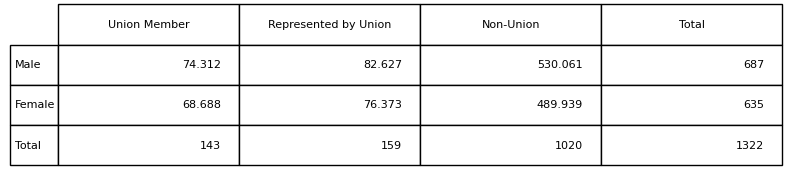
\includegraphics[width=0.75\textwidth]{chi-square-homogenity-ev.png}
    \caption{The compliment to Figure \ref{fig:chi-square-homo}, showing the expected value for each cell. why doesn't matplotlib allow me to export a higher quality image istfg}
    \label{fig:chi-square-homo-ev}
\end{figure}

\textbf{Note that in the expected value table, the row and column sums are still the same, by design.}
From here, you can calculate the test statistic $\chi ^ 2$ and P-value (using df = (number of rows - 1) * (number of cols - 1)) as discussed in section 12.1.
\textbf{Remmber to cite the name of the test ($\chi^2$ test for homogenity),the test statistic, df, and P-value when conducting the test!}

\subsubsection{Chi-square tests for independence}
While chi-square tests for homogenity test \textit{if the distributions of two different populations are the same}, chi-square tests for independence test \textit{if knowing one variable helps predict the value of the other}.
The only functional difference between tests for independence versus homogenity is the hypotheses.
Instead of testing for difference between \textit{two seperate distributions}, tests for independence test for difference between \textit{two seperate variables in the same population}.
That is:
\begin{itemize}
    \item $H_0$: There is no association between x and y in the population.
    \item $H_a$: There is an association between x and y in the population.
\end{itemize}

Other than this, \textit{chi-square tests for independence are calculated exactly the same way as chi-square tests for homogenity}.
There are some differences in the interpertation of each step, but the general process is exactly the same.

\subsubsection{Differences between Homogenity and Independence}
\begin{itemize}
    \item Homogenity tests for if the distribution of \textit{one} categorical variable is the same for \textit{multiple distributions}. Independce tests whether \textit{two} categorical variables are associated in a \textit{single} distribution.
    \item Homogenity tests use data for which \textit{the total sample size for each population is known before the data is collected}. Independence tests use data for which \textit{only the total sample size is known- the size of each population is not known before the data is collected.}
\end{itemize}

\subsection{Inference for Slope}

\end{document}